%%%%%%%%%%%%%%%%%%%%%%%%%%%%% Define Article %%%%%%%%%%%%%%%%%%%%%%%%%%%%%%%%%%
\documentclass{article}
%%%%%%%%%%%%%%%%%%%%%%%%%%%%%%%%%%%%%%%%%%%%%%%%%%%%%%%%%%%%%%%%%%%%%%%%%%%%%%%

%%%%%%%%%%%%%%%%%%%%%%%%%%%%% Using Packages %%%%%%%%%%%%%%%%%%%%%%%%%%%%%%%%%%
\usepackage{listings, xcolor}
\usepackage{parskip}
\usepackage{hyperref}
\usepackage{amsmath}
\usepackage{graphicx}
\usepackage[a4paper, margin = 1.5cm]{geometry}
\usepackage{float}
\usepackage{amsmath}
\usepackage{amssymb}
\usepackage{parskip}
\usepackage{listings}

\lstset{
frame = shadowbox,
basicstyle = \small\ttfamily,
mathescape = true,
numbers = left,
commentstyle = \itshape\color{gray}
columns = flexible,
keepspaces = true,
moredelim = [l]{//}
}

%%%%%%%%%%%%%%%%%%%%%%%%%%%%%% Title & Author %%%%%%%%%%%%%%%%%%%%%%%%%%%%%%%%
\title{Progettazione Architetturale del SW}
\author{Trentin Tommaso}
%%%%%%%%%%%%%%%%%%%%%%%%%%%%%%%%%%%%%%%%%%%%%%%%%%%%%%%%%%%%%%%%%%%%%%%%%%%%%%
\begin{document}
  \maketitle
  \tableofcontents
  \newpage

  \section{Progettazione del SW}
    La progettazione architetturale si colloca nella fase di Progettazione del sistema ed ha un \textbf{ruolo chiave nello sviluppo}, rappresentando il collegamento critico tra ingegneria dei requisiti e progettazione di dettaglio dei componenti.
    \subsection{Finalità}
      Progettare = seguire un processo di risoluzione mirando a descrivere un modo:
      \begin{itemize}
          \item per implementare requisiti funzionali; 
          \item rispettando vincoli dei requisiti non funzionali; 
          \item in conformità con principi di buona qualità.
      \end{itemize}
    \subsection{Decisioni di progettazione}
      Progettista affronta una sereie di problemi di progettazione, ognuno di questi ha normalmente alcune soluzioni alternative (\textbf{design options}). \\ 
      Progettista effettua una serie di \textbf{design decision} oer risolvere il problema scegliendo la \textit{migliore} alternativa possibile in base a requisiti sistema e background / esperienza architetti. \\
      \noindent
        \begin{minipage}[c]{0.38\linewidth}
            \textbf{Design space}: insieme possibili progetti che saranno implementabili scegliendo tra varie alternative.
        \end{minipage}
        \hfill
        \begin{minipage}[c]{0.58\linewidth}
            \centering
            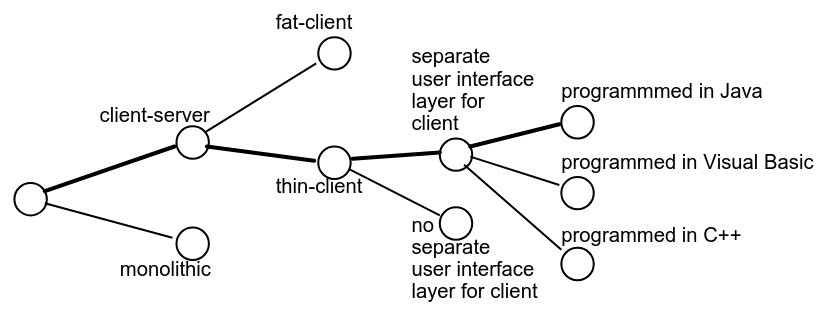
\includegraphics[width=0.8\linewidth]{figures/des_dec.png}
        \end{minipage}
      \subsubsection{Top-Down}
        \begin{itemize}
          \item Si parte da progettazione della struttura ad altissimo livello del sistema, per poi procedere gradualmente più nel dettaglio riguardo aspetti di più basso livello (es. definizione architettura SW e tipo di DB impiegato -> definire formato di dati, algoritmi usati, interfacce utente);
          \item Necessaria per definire una buona struttura per il sistema.
        \end{itemize}
      \subsubsection{Bottom-Up}
        \begin{itemize}
          \item Si parte progettando componenti di basso livello e si decide poi come collegarli per ottenere i componenti di livello più alto; 
          \item Serve a progettare componenti riusabili in altri punti del sistema.
        \end{itemize}
  \section{Progettazione Architetturale}
    Si occupa di comprendere come organizzare il sistema SW e progettarne la sua struttura complessiva, identifica i componenti strutturali di un sistema e le loro relazioni / interfacce; ha come output un modello che descrive l'organizzazione del sistema e la comunicazione tra i suoi componenti.
    \subsection{Architettura, requisiti e prestazioni}
      Architettura SW è importante in quanto influisce (o addirittura pone vincoli) su prestazioni / robustezza / distribuzione / manutenibilità di un sistema. \\ 
      \subsubsection{Requisiti non funzionali e stili architetturali}
        \begin{itemize}
            \item \textbf{Performance}: preferenza per componenti grandi, localizzando operazioni critiche e minimizzando comunicazioni; 
            \item \textbf{Protezione}: utilizzo di architettura a strati, posizionando risorse critiche negli strati interni e ponendo convalide ad ogni strato;
            \item \textbf{Sicurezza funzionale}: concentrazione funzionalità critiche per sicurezza in numero limitato di sottosistemi per fornire meccanismi di protezione riducendo i costi;
            \item \textbf{Disponibilità}: utilizzo di componenti ridondanti e meccanismi per tolleranza ai guasti;
            \item \textbf{Manutenibilità}: utilizzo componenti piccoli facilmente sostituibili / modificabili.
        \end{itemize}
    \subsection{Progettazione architetturale e agilità}
      Attività di progettazione architetturale può scontrarsi con principi agili di \textbf{documentazione minima} e \textbf{refactoring} (possibile rifattorizzare singoli componenti ma per l'intera architettura in quanto ciascun cambiamento può interessare diversi componenti).
    \subsection{Vantaggi progettazione esplicità}
      \begin{itemize}
          \item Fornisce presentazione del sistema ad alto livello che consente confronto tra stakeholders;
          \item Durante progettasione viene analizzata conformità del sistema ai requisiti non funzionali;
          \item Modello può essere riusato per sistemi con requisiti simili.
      \end{itemize}
  \section{Pattern Architetturali}
    \subsection{Concetto di pattern}
      Soluzioni a problemi di progettazione comuni e ricorrenti che si incontrano in applicazioni reali, un pattern architetturale descrive l'organizzazione del sistema che è stata utilizzata in diversi sistemi SW. Vantaggiosi in quanto permettono:
      \begin{itemize}
          \item \textbf{Riuso}
      \end{itemize}
\end{document}

